
\section{Relating Position, Velocity, and Acceleration Graphs\footnote{
1990-93 Dept. of Physics and Astronomy, Dickinson College. Supported by FIPSE
(U.S. Dept. of Ed.) and NSF. Portions of this material may have been modified
locally and may not have been classroom tested at Dickinson College.
}}

Name \rule{2.0in}{0.1pt}\hfill{}Section \rule{1.0in}{0.1pt}\hfill{}Date \rule{1.0in}{0.1pt}

\textbf{Objective }

To understand the relationship between position vs. time, velocity vs. time, and acceleration vs. time
graphs.


\textbf{Introduction} 

The focus of this unit on kinematics is to be able to describe your position, velocity, and acceleration
as a function of time using words and graphs. You will use a motion detector
attached to a computer in the laboratory to learn to describe one-dimensional
motion.

The ultrasonic motion detector sends out a series of sound pulses that are of
too high a frequency to hear. These pulses reflect from objects in the vicinity
of the motion detector and some of the sound energy returns to the detector.
The computer is able to record the time it takes for reflected sound waves to
return to the detector and then, by knowing the speed of sound in air, figure
out how far away the reflecting object is. There are several things to watch
out for when using a motion detector. (1) Do not get closer than 0.15 meters
from the detector because it cannot record reflected pulses which come back
too soon. (2) The ultrasonic waves come out in a cone of about 15\( ^{\circ } \).
It will `see' the closest object. Be sure there is a clear path between the object
whose motion you want to track and the motion detector. (3) The motion detector
is very sensitive and will detect slight changes in motion. 
These changes will appear as bumps in your velocity vs. time graphs.

\vspace{5mm}

\textbf{Apparatus} 

\begin{table}[hbt]
\begin{tabular}{llll}
$\bullet$ & \textit{Science Workshop 750 Interface}  & $\bullet$ & Masking tape for marking distances  \\[3pt]
$\bullet$ & Ultrasonic motion detector               & $\bullet$ & Dynamics cart and track             \\[3pt]
$\bullet$ & \textit{DataStudio} software             & $\bullet$ & Lab stand to incline the track      \\[3pt]
$\bullet$ & Wooden board                             &                                                 \\[3pt]
\end{tabular}
\end{table}

\textbf{Position vs. Time Graphs of Your Motion }

The purpose of this activity is to learn how to relate graphs of position as a function
of time to the motions they represent. How does a position vs. time graph look
when you move slowly? Quickly? What happens when you move toward the motion
detector? Away? After completing the next few activities, you should be able
to look at a position vs. time graph and describe the motion of the object and sketch a graph
representing that motion.

Note that the motion detector measures the distance of an object from the detector,
and that the motion detector is located at the origin of each graph. It is common
to refer to the distance of an object from some origin as the position of the
object. Therefore, it is better to refer to these graphs as position vs. time
graphs than distance vs. time graphs.


\textbf{Activity \stepcounter{activity}\arabic{activity}: Making Position vs. Time Graphs }\actlabel{actone}

In this Activity you will measure your own movements with the motion sensor.
You can try to glide smoothly
along the floor, but don't be surprised to see small bumps in velocity graphs.
Also, some objects like bulky sweaters are good sound absorbers and may not be
``seen'' well by a motion detector. You may want to hold a book
or a board in front of you if you have loose clothing on.

You will use the \textit{DataStudio} software to do the following activities.
For Activity 1 launch the \textbf{Position
Graphs} application by going to \textbf{Start} $\rightarrow$ \textbf{Programs} $\rightarrow$ \textbf{Physics Applications} $\rightarrow$ \textbf{131 Workshop} $\rightarrow$ \textbf{Position Graphs}. To start a data run, click the \textbf{Start} button. To stop a data run,
click the \textbf{Stop} button. After a data run, the graph can be expanded
by clicking on the \textbf{Scale to fit} button in the upper left corner of
the Graph window. Multiple data sets can be displayed on the same graph. Data
can be removed from the graph by selecting \textbf{Delete Last Data Run} or
\textbf{Delete All Data Runs} from the \textbf{Experiment} menu. When you are
finished with the activities, choose \textbf{Quit} from the \textbf{File} menu
and do not save this activity.
See the Appendix for more details on using {\it DataStudio}.

Before you begin the activities, you should mark a position scale on the floor.
To do this, position one person at approximately 1 meter in front of the motion
detector and take data for 1 second. The computer will display a horizontal
line showing the position measured by the detector. The person standing in front
of the detector should then adjust his/her position and the procedure repeated
until the 1 meter position is established. Mark the 1 meter position on the
floor with a piece of masking tape and then mark the 2, 3 and 4 meter positions
using the 2 meter stick.

Make position-time graphs for the following motions and sketch the graph you
observe in each case:

\begin{enumerate}

\item Starting at 0.5 m, walk away from the origin (i.e., the detector) slowly
and steadily.

\vspace{0.3cm}
{\par\centering 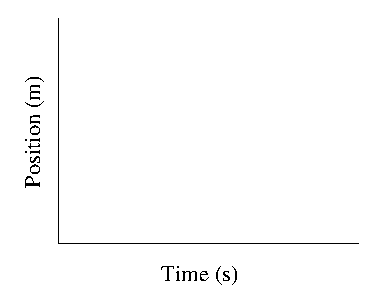
\includegraphics{iqsRelatingMotion/position_fig1.eps} \par}
\vspace{0.3cm}

\item Walk toward the detector (origin) quickly and steadily.

\vspace{0.3cm}
{\par\centering 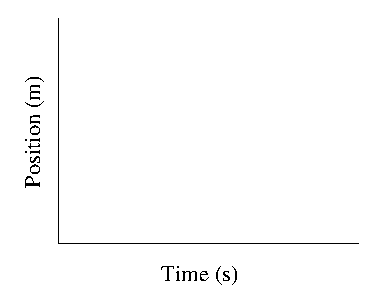
\includegraphics{iqsRelatingMotion/position_fig1.eps} \par}
\vspace{0.3cm}

\item Describe the difference between the graph made by walking toward and the
one made walking away from the motion detector.
\vspace{20mm}

\end{enumerate}

\newpage

\textbf{Activity \stepcounter{activity}\arabic{activity}: Predicting Velocity Graphs from Position Graphs}\actlabel{acttwo}

\begin{enumerate}

\item Carefully study the position graph shown below and predict the velocity
vs. time graph that would result from the motion. Using a dashed line, sketch
your prediction of the corresponding velocity vs. time graph on the velocity
axes.

\vspace{0.3cm}
{\par\centering 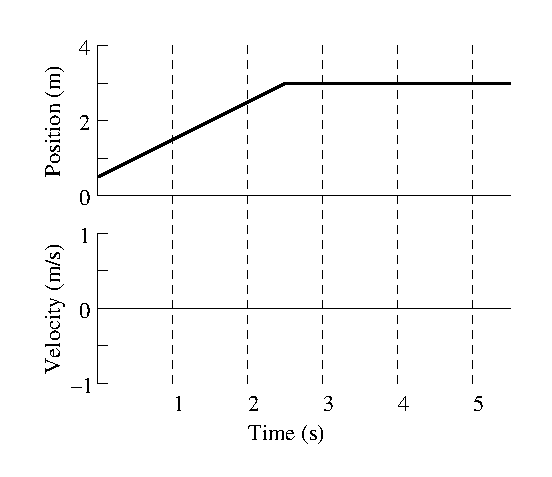
\includegraphics{iqsRelatingMotion/relating_fig1.eps} \par}
\vspace{0.3cm}

\item After each person in your group has sketched a prediction, test your prediction
by walking and matching the position vs. time graph shown. 
To explore how position vs. time and velocity vs. time graphs are related, 
go to \textbf{Start} $\rightarrow$ \textbf{Programs} $\rightarrow$ \textbf{Physics Applications} $
\rightarrow$ \textbf{131 Workshop} $\rightarrow$ \textbf{Position \& Velocity Graphs}.
When you have made a good duplicate
of the position graph, sketch your actual graph over the existing position vs.
time graph.
Use a solid line to draw the actual velocity graph on the same graph with
your prediction. (Do not erase your prediction).

\item How would the position graph be different if you moved faster? Slower? 
\vspace{20mm}

\item How would the velocity graph be different if you moved faster? Slower? 
\vspace{20mm}

\end{enumerate}

\newpage

\textbf{Activity \stepcounter{activity}\arabic{activity}: Finding Position from a Velocity Graph }\actlabel{actthree}

\begin{enumerate}

\item Carefully study the velocity graph that follows. Using a dashed line, sketch your prediction of the corresponding position graph on the top set of axes.
(Assume that you started at the 1-meter mark.)

\vspace{0.3cm}
{\par\centering 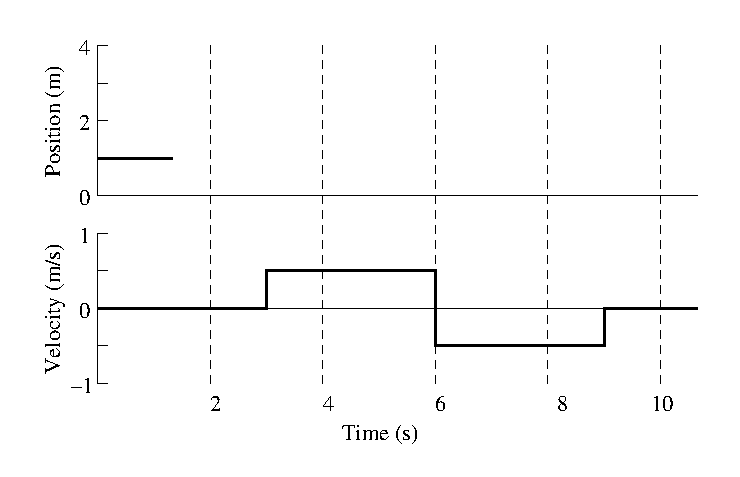
\includegraphics{iqsRelatingMotion/relating_fig2.eps} \par}
\vspace{0.3cm}

\item After each person has sketched a prediction, do your group's best to duplicate the bottom (velocity vs. time) graph by walking. 
When you have made a good duplicate of the velocity vs. time graph, draw your actual result over the existing velocity vs. time graph. 
Use a solid line on the top graph to draw the actual position vs. time graph on the same axes with your prediction. Do not erase your prediction.

\item How can you tell from a velocity vs. time graph that the moving object has
changed direction?
\vspace{10mm}

\item What is the velocity at the moment the direction changes? 
\vspace{10mm}

\item Is it possible to actually move your body (or an object) to make vertical
lines on a position vs. time graph? Why or why not? What would the velocity
be for a vertical section of a position vs. time graph? 
\vspace{10mm}

\item How can you tell from a position vs. time graph that your motion is steady
(motion at a constant velocity)? 
\vspace{10mm}

\item How can you tell from a velocity vs. time graph that your motion is steady
(constant velocity)? 
\vspace{10mm}

\end{enumerate}

\newpage

\textbf{Activity \stepcounter{activity}\arabic{activity}: Position, Velocity and Acceleration Graphs of Constant Velocity}\actlabel{actfour}

In order to get a feeling for acceleration, it is helpful to create and learn
to interpret velocity vs. time and acceleration vs. time graphs for some relatively
simple motions of a cart on a track. 
The cart's motion on a track is simpler than the more complex movements associated with walking.
You will be observing the cart with the
motion detector as it moves at a constant velocity and as it changes its velocity
at a constant rate. Use the \textbf{P, V \& A Graphs} application by going to
\textbf{Start} $\rightarrow$ \textbf{Programs} $\rightarrow$ \textbf{Physics Applications} 
$\rightarrow$ \textbf{131 Workshop} $\rightarrow$ \textbf{P, V \& A Graphs} for these activities.

\begin{enumerate}

\item Based on your observations of the motions of your body in the last Activity,
how should the position and velocity graphs look if you move the cart at a constant
velocity away from the motion detector starting at the 0.5 meter mark? Sketch
your predictions with dashed lines on the axes that follow.

%\vspace{0.3cm}
{\par\centering 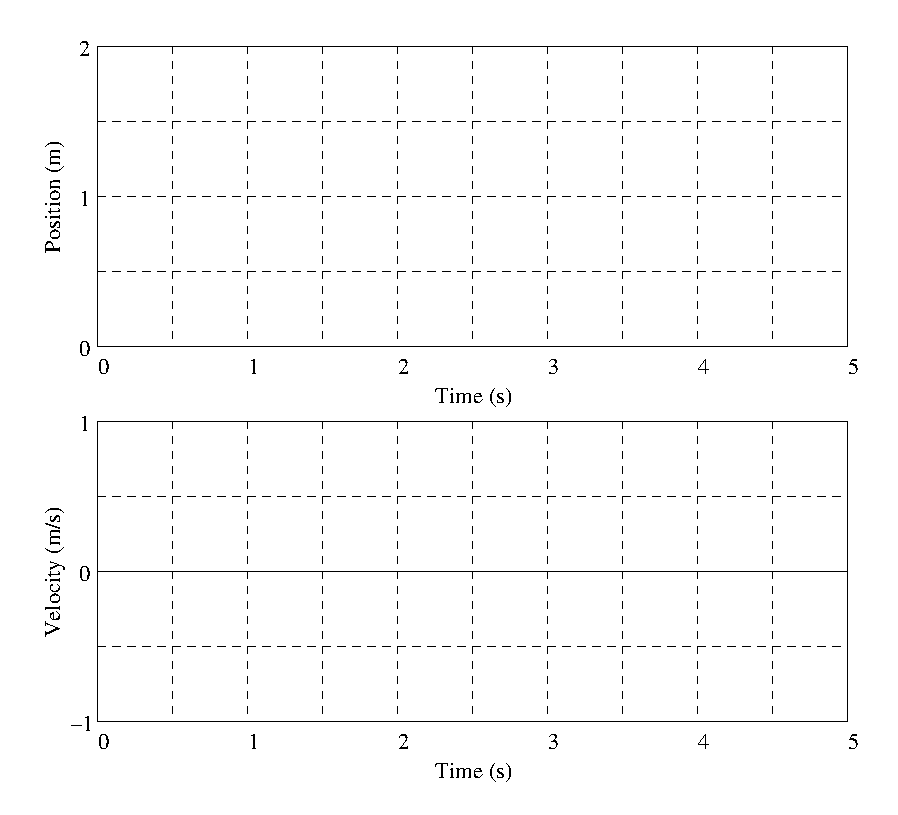
\includegraphics[width=4.75in]{iqsRelatingMotion/changing_fig1.eps} \par}
\vspace{0.1cm}

\item Acceleration is defined as the time rate of change of velocity. Sketch your
prediction of the cart acceleration on the axes that follow using a dashed line.

%\vspace{0.3cm}
{\par\centering 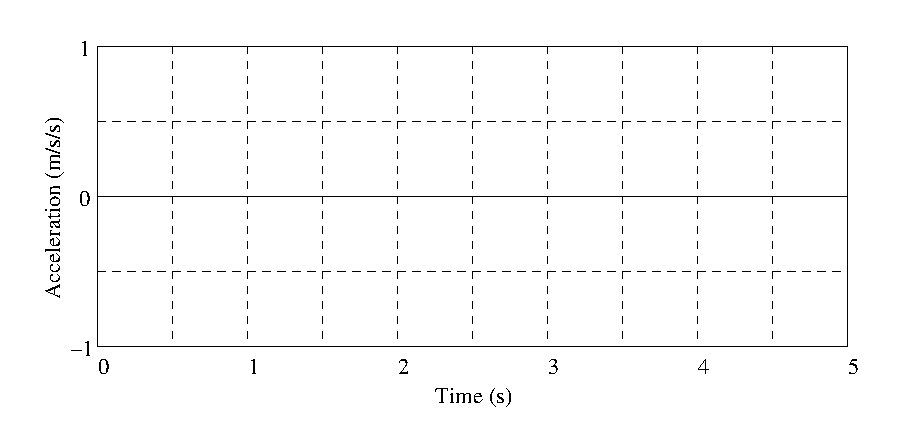
\includegraphics[width=4.75in]{iqsRelatingMotion/changing_fig2.eps} \par}
\vspace{0.1cm}

\item Test your prediction. Be sure that the cart is never closer than 0.15 meter
from the motion detector. Try several times until you get a fairly constant
velocity. Sketch your results with solid lines on the axes shown above. The
acceleration vs. time graphs will exhibit small fluctuations due to irregularities
in the motion of the cart. You should ignore these fluctuations and draw smooth
patterns.

\item Did your graphs agree with your predictions? What characterizes constant
velocity motion on a position vs. time graph? 
\vspace{10mm}

\item What characterizes constant velocity motion on a velocity vs. time graph?
\vspace{10mm}

\item What characterizes constant velocity motion on an acceleration vs. time graph?
\vspace{10mm}

\end{enumerate}

\textbf{Speeding Up at a Moderate Rate} 

In the next activity you will look at velocity and acceleration graphs of the
motion of a cart when its velocity is changing. You will be able to see how
these two representations of the motion are related to each other when the cart
is speeding up.
In order to get your cart speeding up smoothly use the lab stand to raise the
track several centimeters at the end where the motion detector is mounted.

\textbf{Activity \stepcounter{activity}\arabic{activity}: Graphs Depicting Speeding Up}\actlabel{actsix}

\begin{enumerate}

\item Predict the shape of the position, velocity, and acceleration vs. time graphs
for the cart moving away from the sensor and speeding up. Sketch your predictions
on the following axes using dashed lines.

\vspace{0.3cm}
{\par\centering 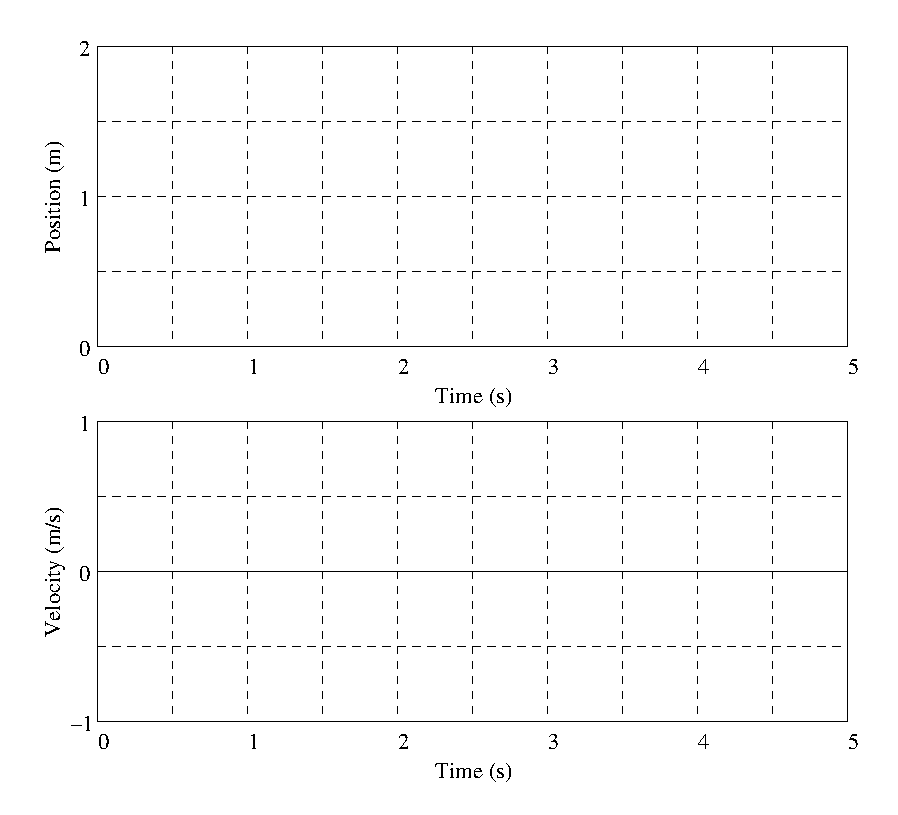
\includegraphics[width=4.75in]{iqsRelatingMotion/changing_fig1.eps} \par}
\vspace{0.3cm}

\vspace{0.3cm}
{\par\centering 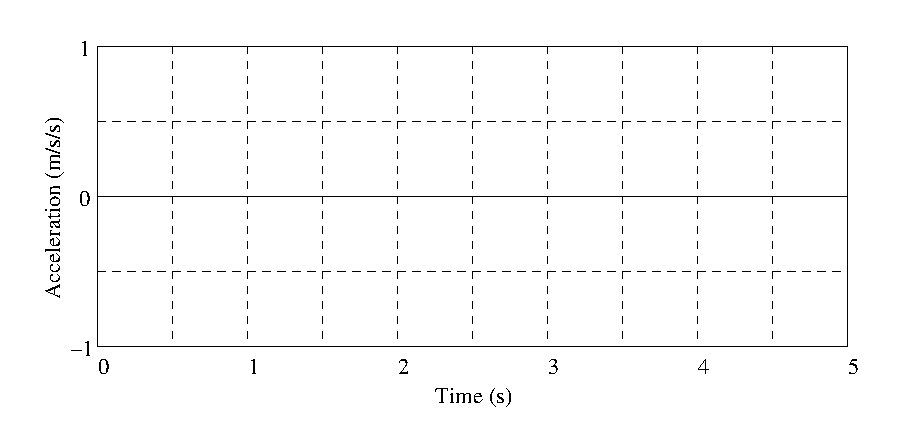
\includegraphics[width=4.75in]{iqsRelatingMotion/changing_fig2.eps} \par}
\vspace{0.3cm}

\item Create graphs of the motion of your cart as it moves away from the detector
and speeds up. Sketch the graphs neatly on the above axes using solid lines.

\item How does your position graph differ from the position graphs for steady
(constant velocity) motion? 
\vspace{13mm}

\item What feature of your velocity graph signifies that the motion was away from
the detector? 
\vspace{13mm}

\item What feature of your velocity graph signifies that the cart was speeding
up? How would a graph of motion with a constant velocity differ? 
\vspace{13mm}

\item During the time that the cart is speeding up, is the acceleration positive
or negative? How does speeding up while moving away from the detector result
in this sign of acceleration? Hint: Remember that acceleration is the rate of
change of velocity. Look at how the velocity is changing.\customlabel{posneg}{6}
\vspace{13mm}

\item How does the velocity vary in time as the cart speeds up? Does it increase
at a steady rate or in some other way? 
\vspace{13mm}

\item How does the acceleration vary in time as the cart speeds up? Is this what
you expect based on the velocity graph? Explain.
\vspace{13mm}

\end{enumerate}

\newpage

\textbf{Homework} 

\begin{enumerate}

\item To find the average acceleration of the cart during some time interval (the
average time rate of change of its velocity), you must measure its velocity
at two different times, calculate the difference between the final value and
the initial value and divide by the time interval.
Calculate the average acceleration during some time interval from your velocity graph in Activity \ref{actfour}.  
Does the result agree with your acceleration graph in Activity \ref{actfour}?
\vspace{20mm}

\item The diagram below shows the positions of the cart at equal time intervals.
(This is like taking snapshots of the cart at equal time intervals.) At each
indicated time, sketch a vector above the cart which might represent the velocity
of the cart at that time while it is moving at a constant velocity away from
the motion detector.

\vspace{0.3cm}
{\par\centering 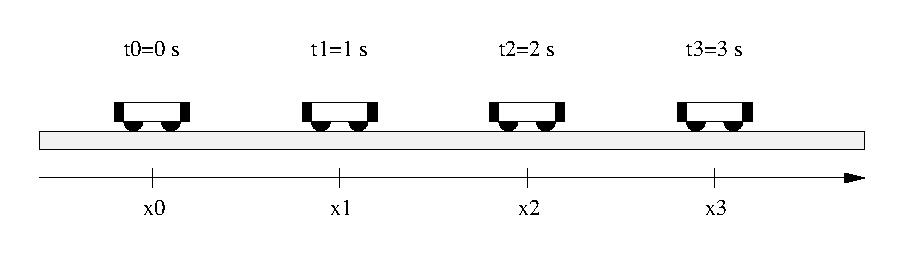
\includegraphics{iqsRelatingMotion/changing_fig3.eps} \par}
\vspace{0.3cm}

\item Explain how you would find the vector representing the change in velocity
between the times 1.0~s and 2.0~s in the diagram above. From this vector, what
value would you calculate for the acceleration? Explain. Is this value in agreement
with the acceleration graph you obtained in Activity \ref{actfour}?
\vspace{20mm}


\item  The diagram below shows the positions of the cart at equal time intervals.
At each indicated time, sketch a vector above the cart which might represent
the velocity of the cart at that time while it is moving away from the motion
detector and speeding up.

\vspace{0.3cm}
{\par\centering 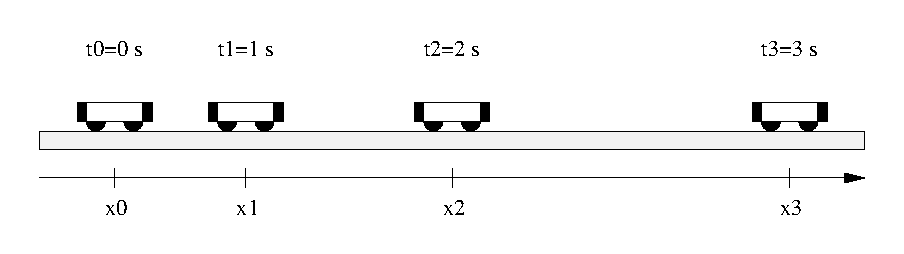
\includegraphics{iqsRelatingMotion/changing_fig4.eps} \par}
\vspace{0.3cm}

\newpage

Show below how you would find the approximate length and direction of the
vector representing the change in velocity between the times 1.0~s and 2.0~s
using the diagram above. No quantitative calculations are needed. Based on the
direction of this vector and the direction of the positive x-axis, what is the
sign of the acceleration? Does this agree with your answer to Activity \ref{actsix}.\ref{posneg}?
\vspace{20mm}

\item Draw the velocity graphs for an object whose motion produced the position-time
graphs shown below on the left. Position is in meters and velocity in meters
per second. Note: Unlike most real objects, you can assume these objects can
change velocity so quickly that it looks instantaneous with this time scale.

%\vspace{0.3cm}
%{\par\centering 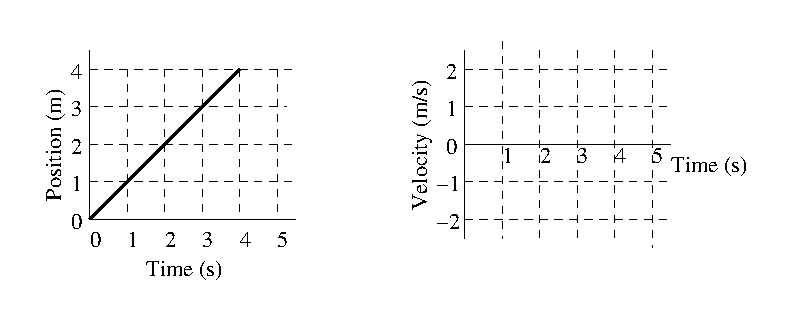
\includegraphics{iqsRelatingMotion/relating_fig3.eps} \par}
%\vspace{0.3cm}

\vspace{0.3cm}
{\par\centering 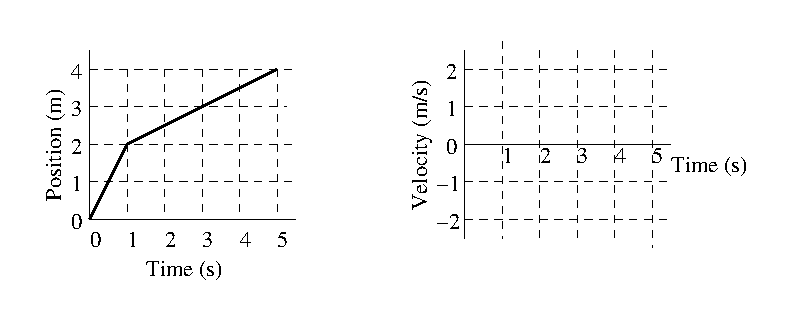
\includegraphics{iqsRelatingMotion/relating_fig4.eps} \par}
\vspace{0.3cm}

\vspace{0.3cm}
{\par\centering 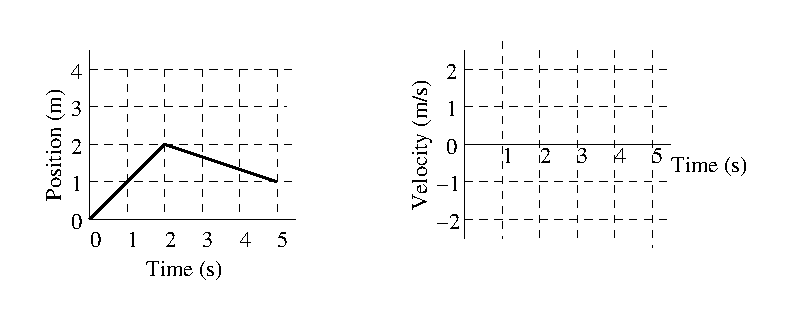
\includegraphics{iqsRelatingMotion/relating_fig5.eps} \par}
\vspace{0.3cm}

\newpage

\item Draw careful graphs below of position and velocity for a cart that (a) moves
away from the origin at a slow and steady (constant) velocity for the first
5 seconds; (b) moves away at a medium-fast, steady (constant) velocity for the
next 5 seconds; (c) stands still for the next 5 seconds; (d) moves toward the
origin at a slow and steady (constant) velocity for the next 5 seconds; (e)
stands still for the last 5 seconds.

\vspace{0.3cm}
{\par\centering 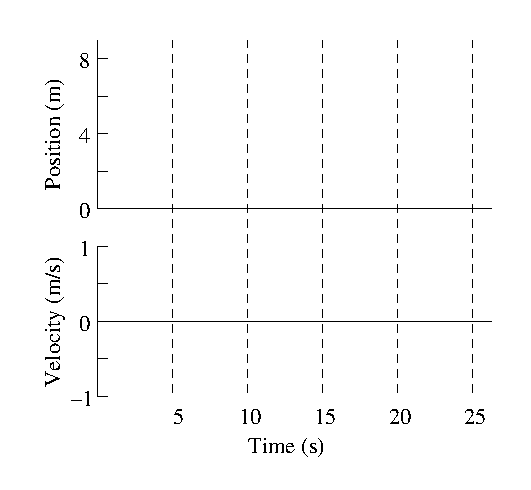
\includegraphics{iqsRelatingMotion/relating_fig6.eps} \par}
\vspace{0.3cm}


\item An object moving along a line (the + position axis) has the acceleration-time
graph shown below. Describe how might the object move to create this graph if
it is moving away from the origin?

\vspace{0.3cm}
{\par\raggedright 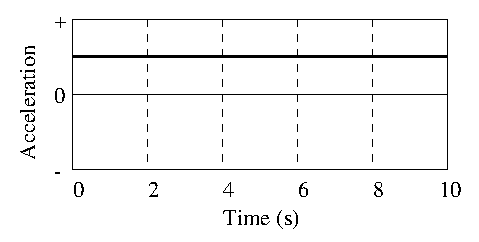
\includegraphics{iqsRelatingMotion/changing_fig6.eps} \par}
\vspace{1.3cm}

\item Sketch on the axes below a velocity-time graph that goes with the above acceleration-time
graph.

\vspace{0.3cm}
{\par\centering 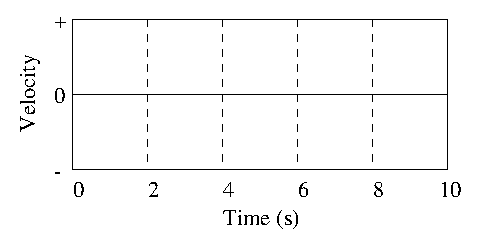
\includegraphics{iqsRelatingMotion/changing_fig7.eps} \par}
\vspace{1.3cm}

\item For each of the velocity-time graphs below, sketch the shape of the acceleration-time
graph that goes with it.

\vspace{0.3cm}
{\par\centering 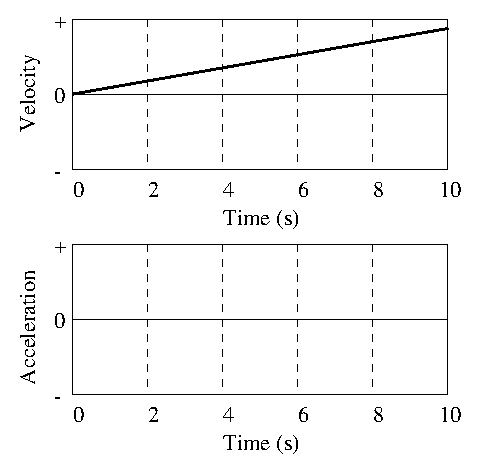
\includegraphics{iqsRelatingMotion/changing_fig8.eps} \par}
\vspace{0.3cm}

\vspace{0.3cm}
{\par\centering 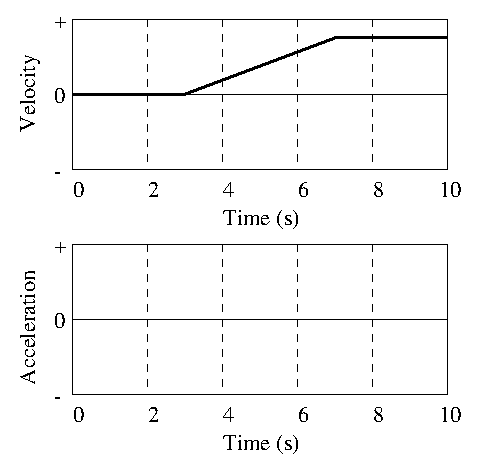
\includegraphics{iqsRelatingMotion/changing_fig9.eps} \par}
\vspace{0.3cm}

%\item The following is a velocity-time graph for a car.

%\vspace{0.3cm}
%{\par\centering 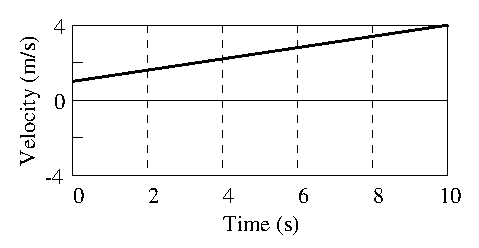
\includegraphics{iqsRelatingMotion/changing_fig10.eps} \par}
%\vspace{0.3cm}

%What is the average acceleration of the car? Show your work below.
%\vspace{30mm}

\item Which position-time graph below could be that for a cart that is steadily
accelerating away from the origin?

\vspace{0.3cm}
{\par\centering 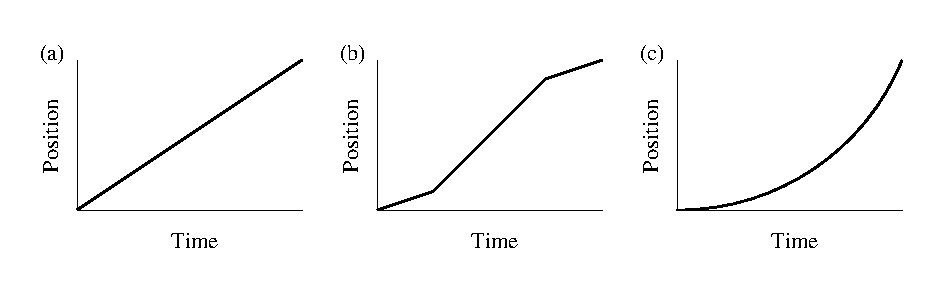
\includegraphics{iqsRelatingMotion/changing_fig11.eps} \par}
\vspace{0.3cm}


\item A car can move along a line (the + position axis). Sketch velocity-time and
acceleration-time graphs which correspond to each of the following descriptions
of the car's motion.
The car starts from rest and moves away from the origin increasing its speed
at a steady rate.

\vspace{0.3cm}
{\par\centering 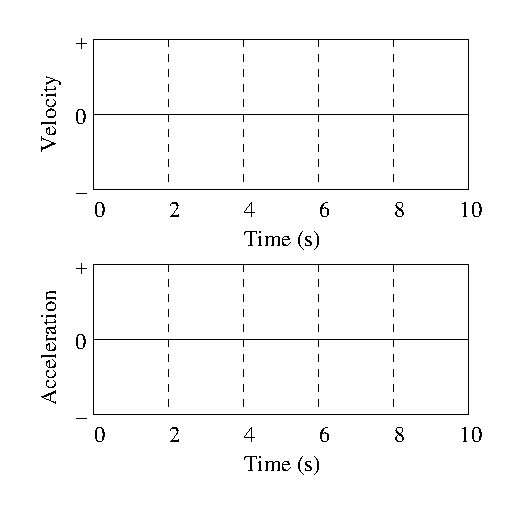
\includegraphics{iqsRelatingMotion/changing_fig12.eps} \par}
\vspace{0.3cm}

\item The same car is moving away from the origin at a constant velocity.

\vspace{0.3cm}
{\par\centering 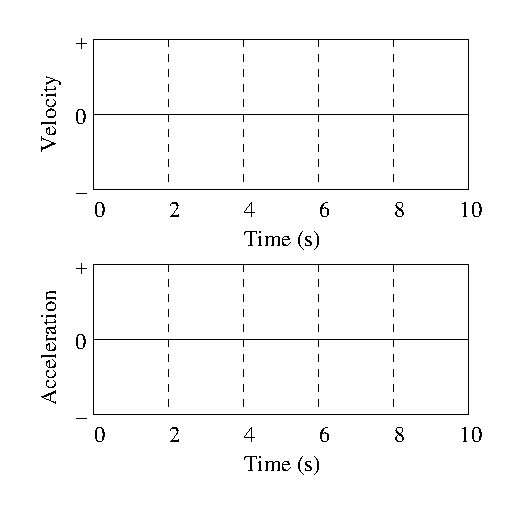
\includegraphics{iqsRelatingMotion/changing_fig12.eps} \par}
\vspace{0.3cm}

%\item The car starts from rest and moves away from the origin increasing its speed
%at a steady rate twice as large as in (6) above.

%\vspace{0.3cm}
%{\par\centering 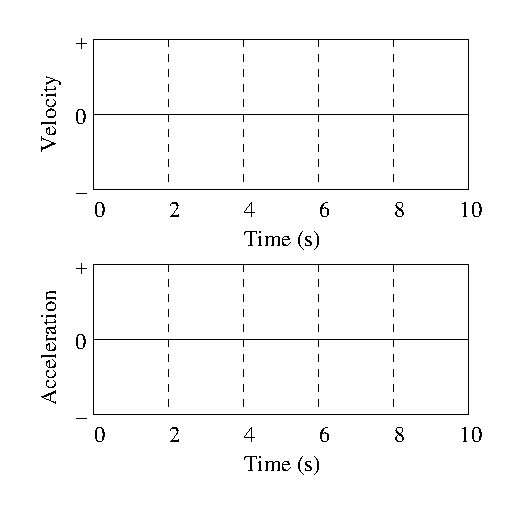
\includegraphics{iqsRelatingMotion/changing_fig12.eps} \par}
%\vspace{0.3cm}

%\item The car is moving away from the origin at a constant velocity twice as large
%as in (7) above.

%\vspace{0.3cm}
%{\par\centering 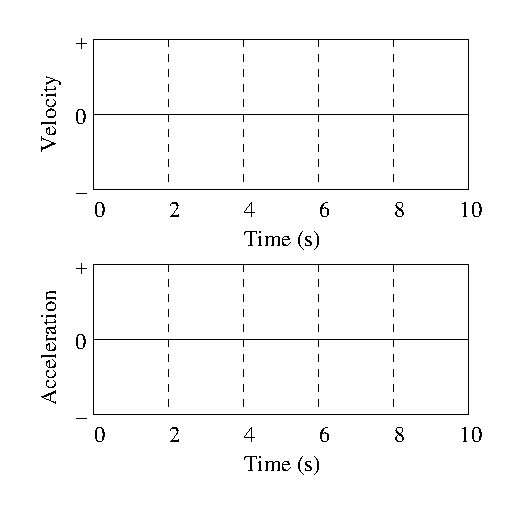
\includegraphics{iqsRelatingMotion/changing_fig12.eps} \par}
%\vspace{0.3cm}

\end{enumerate}
